\documentclass[12pt,journal,compsoc]{IEEEtran}
\usepackage[utf8]{inputenc}
\usepackage{hyperref} 
\usepackage{fancyhdr}

\usepackage{graphicx}



\begin{document}

\title{Game Title \\ Design Document}

\author{Bjørn~Fjukstad \\ BIO-8010 Communicating Science Module 3\\ Visualizing
your science \\ \url{github.com/fjukstad/bio-8010}} 

\maketitle
\vspace{-15mm}

\section{Introduction} 
Code Lab is a game where kids collaborate on escaping from an underground
dungeon by programming their in-game characters to fight monsters, solve puzzles
and collect gems. The game is played in a collaborative environment such as the
Tromsø Display Wall\cite{anshus2013nineyears}, where kids program on their own
devices and run the game on the large display. The display wall environment
provides an interactive arena where kids can collaborate on completing the game
together.

Since the kids need to program the characters to perform different tasks, they
will have to learn the basics of programming. The different levels will require
them to learn about \emph{variables}, \emph{data structures}, \emph{functions}
and \emph{control statements} such as \emph{for}-loops and \emph{if}-statements. 
As the kids play the game, the puzzles and problems they are faced with will
increase in difficulty, making it necessary to design and implement more
complex solutions. 

The game is intended for children 10 - 16 years old, who already have some
experience with graphical programming environments such as
Scratch\cite{resnick2009scratch}. It is intended for kids that want to learn
more about programming, specifically getting started with text-based
programming. 

CodeLab is open-sourced at \url{github.com/fjukstad/bio-8010}. 

% Structure
%\subsection{Concept, Goal and Learning Goals} 
%\subsection{Target Audience} 

\section{Description} 
CodeLab takes place in a fictional dungeon, where each player is assigned a
hero that he or she controls by programming their actions. The players equip
their heroes with armor, weapons and other items that can help them complete the
different levels. For each level, the players have to complete a set of tasks by
programming their characters by using a programming language similar to the 
Lua programming language\footnote{\url{lua.org}}. Players 
write the code on their local machine, be it a laptop or a smart phone, and see
their characters perform the actions on a large shared display. Alongside the
game view, the players see each others code making it possible to help out
eachother if they encounter any problems. 
\begin{figure}[htb]
    \begin{centering}
    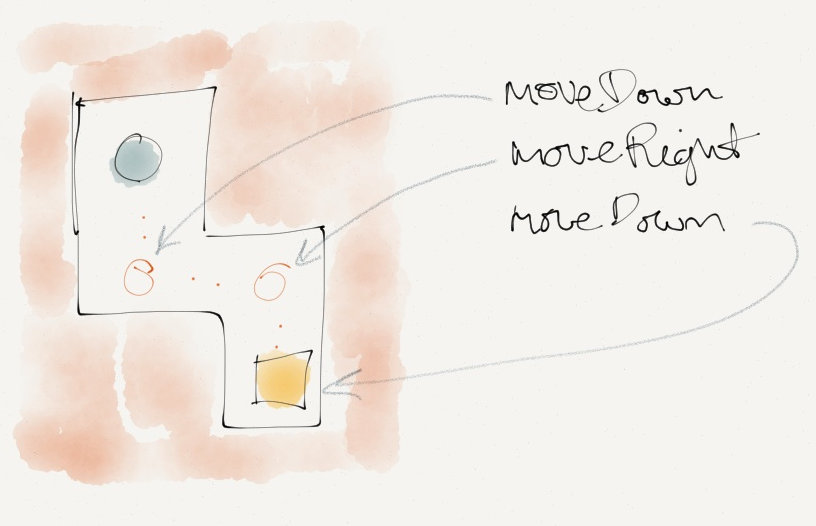
\includegraphics[width=0.4\textwidth]{./figures/codelab3.png}
    \caption{A sketch of the first level of CodeLab. The goal of the level
    is to write code that moves the character (the circle) down to the
    yellow square. The player writes three commands, $moveDown$,
    $moveRight$ and $moveDown$ to complete the level. } 
    \label{fig:level1}
    \end{centering} 
\end{figure}


\begin{figure}[htb]
    \begin{centering}
    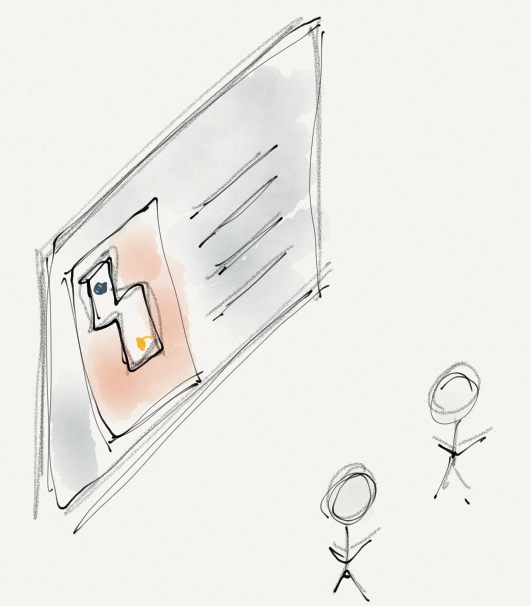
\includegraphics[width=0.4\textwidth]{./figures/codelab2.png}
    \caption{The CodeLab environment. Players collaborate to solve a level. Both
    the graphical window where the game runs, as well as the source code is
    shown on a large display. } 
    \label{fig:environ}
    \end{centering} 
\end{figure}

\begin{figure}[htb]
    \begin{centering}
    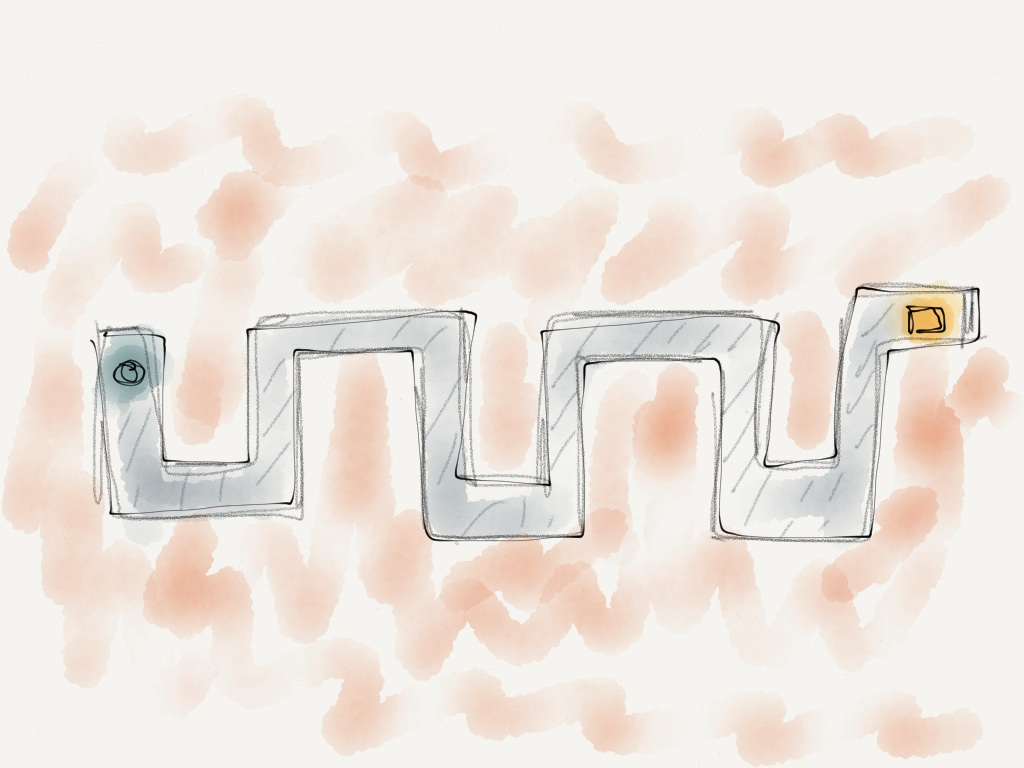
\includegraphics[width=0.4\textwidth]{./figures/codelab4.jpg}
    \caption{A level that can be completed by writing a simple loop.} 
    \label{fig:loop}
    \end{centering} 
\end{figure}

\begin{figure}[htb]
    \begin{centering}
    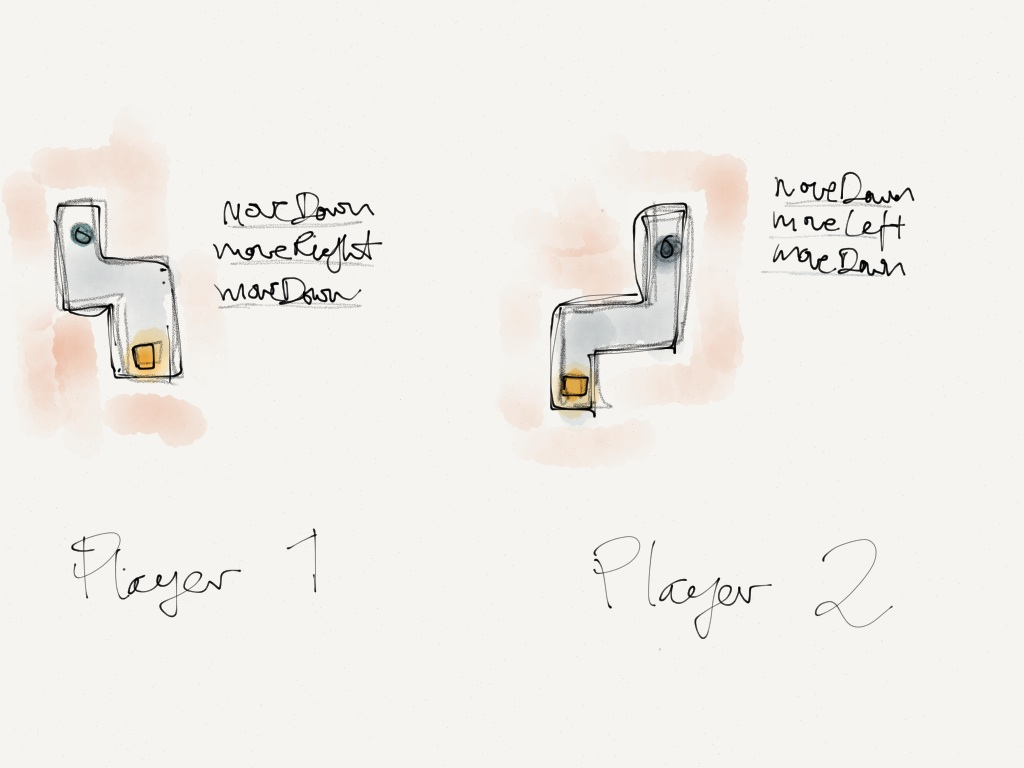
\includegraphics[width=0.4\textwidth]{./figures/codelab5.jpg}
    \caption{Two players trying to complete the first level. This view is shown
    on the large display, where they can help each other write the necessary
    code. } 
    \label{fig:loop}
    \end{centering} 
\end{figure}




\subsection{Game Narrative} 


\subsection{Game Setting} 
\subsection{Game Tasks} 

\section{Key features} 
\subsection{Game Mechanics} 
\subsection{Progression} 
\subsection{Reward and Motivation} 
\subsection{Balancing} 

\section{Platform} 
\subsection{Art} 
\subsection{Music and Audio}

\section{Production and Team} 
\section{Competition and Inspiration}


% Fetch your references, in a file called report.bib
\bibliography{design-document}{}
\bibliographystyle{plain}
\end{document} 
